%-------------------------------------------------------------------------------
% seq24_pattern_editor
%-------------------------------------------------------------------------------
%
% \file        seq24_pattern_editor.tex
% \library     Documents
% \author      Chris Ahlstrom
% \date        2015-07-19
% \update      2015-07-22
% \version     $Revision$
% \license     $XPC_GPL_LICENSE$
%
%     Provides the concepts.
%
%-------------------------------------------------------------------------------

\section{Pattern Editor}
\label{sec:seq24_pattern_editor}

   The \textsl{Seq24 Pattern Editor} is used to edit and preview a pattern,
   as well as to configure its buss and channel settings.

\begin{figure}[H]
   \centering 
   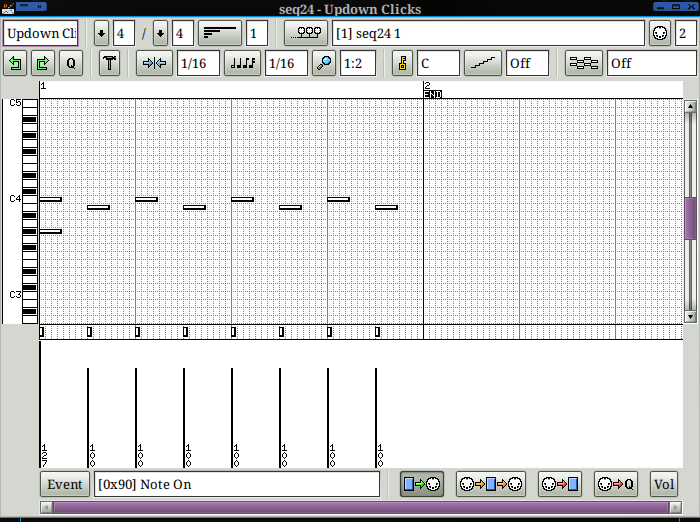
\includegraphics[scale=0.75]{pattern/pattern-edit-window.png}
   \caption{Pattern Edit Window}
   \label{fig:pattern_edit_window}
\end{figure}

   This dialog is quite complex.
   For exposition, we break it into a first panel, a second panel, a
   bottom panel, and a piano-roll/events section.

   \begin{enumber}
      \item \textbf{First Panel}
      \item \textbf{Second Panel}
      \item \textbf{Piano-Roll/Events Panel}
      \item \textbf{Bottom Panel}
   \end{enumber}

\subsection{Pattern Editor / First Panel}
\label{subsec:seq24_pattern_editor_first}

   The top bar of the Pattern (sequence) Editor lets you change the name of
   the pattern, the time signature of the piece, how long the loop is, and
   some other configuration items.

\begin{figure}[H]
   \centering 
   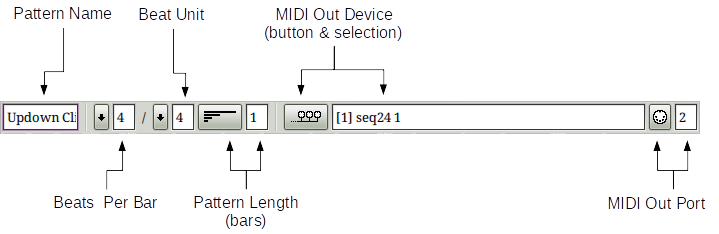
\includegraphics[scale=0.75]{pattern/pattern-edit-first-panel-items.png}
   \caption{Pattern Editor, First Panel Items}
   \label{fig:pattern_editor_first_panel_items}
\end{figure}

   \begin{enumber}
      \item \textbf{Pattern Name}
      \item \textbf{Beats Per Bar}
      \item \textbf{Beat Unit}
      \item \textbf{Pattern Length}
      \item \textbf{MIDI Out Device}
      \item \textbf{MIDI Out Port}
   \end{enumber}

   \setcounter{ItemCounter}{0}      % Reset the ItemCounter for this list.

   \itempar{Pattern Name}{pattern editor!name}
   Provides the name of the pattern.
   This name should be short and memorable.
   It is displayed in the Patterns window.

   \itempar{Beats Per Bar}{pattern editor!beats/bar}
   Part of the time signature, and specifies the number of beat units per bar.
   The possible values range from 1 to 16.

   \itempar{Beat Unit}{pattern editor!beat unit}
   Part of the time signature, and specifies the size of the beat unit:
   1 for whole notes; 2 for half notes; 4 for quarter notes; 8 for eight notes;
   and 16 for sixteenth notes.

   \itempar{Pattern Length}{pattern editor!progress}
   Sets the length of the current pattern, in measures.
   The possible values range from 1 to 16, then 32, and 64.

   \textsl{(It would sure be nice to have a value that represents
   "indefinite", so that the loop or pattern would be more like a track,
   and perhaps not be repeatable.)}

   \itempar{MIDI Out Device}{pattern editor!midi out device}
   This setting specifies one of the 16 MIDI output busses provided by
   \textsl{Seq24}.  The settings look a lot like
   \figureref{fig:pattern_window_right_click_midi_bus}.

   \itempar{MIDI Out Port}{pattern editor!midi out port}
   This settings select the MIDI output channel, or port.
   The possible values range from 1 to 16.

\subsection{Pattern Editor / Second Panel}
\label{subsec:seq24_pattern_editor_second}

   The second panel of the Pattern Editor provides a number of additional
   settings.

\begin{figure}[H]
   \centering 
   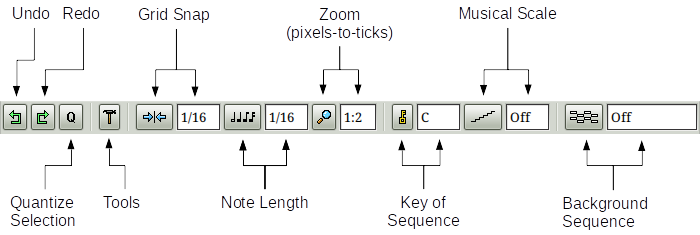
\includegraphics[scale=0.75]{pattern/pattern-edit-second-panel-items.png}
   \caption{Pattern Editor, Second Panel Items}
   \label{fig:pattern_editor_main_panel_items}
\end{figure}

   \begin{enumber}
      \item \textbf{Undo}
      \item \textbf{Redo}
      \item \textbf{Quantize Selection}
      \item \textbf{Tools}
      \item \textbf{Grid Snap}
      \item \textbf{Note Length}
      \item \textbf{Zoom}
      \item \textbf{Key of Sequence}
      \item \textbf{Musical Scale}
      \item \textbf{Background Sequence}
   \end{enumber}

   \setcounter{ItemCounter}{0}      % Reset the ItemCounter for this list.

   \itempar{Undo}{pattern editor!undo}
   The Undo button will roll back any changes to the pattern from this
   session.
   It will roll back one change each time it is pressed.
   It is not certain what the undo limit is, however.
   \index{keys!ctrl-z}
   Pressing \texttt{Ctrl-Z} is the same as using the \textbf{Undo} button.

   \itempar{Redo}{pattern editor!redo}
   The Redo button will restore any undone changes to the pattern from this
   session.
   It will restore one change each time it is pressed.
   It is not certain what the redo limit is, however.
   There doesn't seem to be a "Redo" key.

   \itempar{Quantize Selection}{pattern editor!quantize}
   Pressing this button will quantize the selected events, presumably as per
   the \textbf{Grid Snap} setting.

   \itempar{Tools}{pattern editor!tools}
   This button brings up a nested menu of tools for modifying selected
   events and notes.

\begin{figure}[H]
   \centering 
   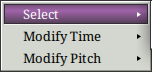
\includegraphics[scale=0.75]{pattern/tools-first-menu.png}
   \caption{Tools Context Menu}
   \label{fig:pattern_editor_tools_first_menu}
\end{figure}

   \begin{enumber}
      \item \textbf{Select}
      \item \textbf{Modify Time}
      \item \textbf{Modify Pitch}
   \end{enumber}

   $\bullet$ \textbf{Select} provides two sets of selections for notes:
   \begin{itemize}
      \item \textbf{All Notes}, which selects all notes in the pattern;
         Note that \index{keys!ctrl-a} \texttt{Ctrl-A} will also select
         all of the events in the pattern editor.
      \item \textbf{Inverse Notes}, which inverts the selection of notes.
   \end{itemize}

   Other event-selection actions are provided:

   \begin{itemize}
      \item \index{left click}
         Pressing the left button on a note or a event deselects all other
         notes or events, and selects the item clicked on.
      \item \index{ctrl left click}
         Pressing the \texttt{Ctrl} key and the left button on a note or a
         event \textsl{adds} that event to the selection.
      \item \index{left click drag}
         Pressing the left mouse button and dragging also lets one
         select multiple events and notes.
      \item \index{ctrl left click drag}
         Pressing the \texttt{Ctrl} while left-click+dragging lets one
         make additional selections of multiple events and notes.
   \end{itemize}

   $\bullet$ \textbf{Modify Time} offers two ways to tweak the timing of the
   selected note:
   \textbf{Quantize Selected Notes}, which quantizes the selected
   notes, presumably the same way as the \textbf{Quantize} ("\textbf{Q}")
   button; \textbf{Tighten Selected Notes}, which presumably is a less
   strict form of quantization.
   TODO: \index{"todo!what is tighten"} Need more information about this.

   $\bullet$ \textbf{Modify Pitch} has only one entry,
   \textbf{Transpose Selected},
   which brings up the following sub-menu:

\begin{figure}[H]
   \centering 
   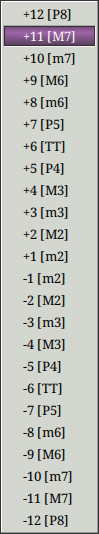
\includegraphics[scale=0.75]{pattern/tools-transpose-selected-menu.png}
   \caption{Tools Transpose Selected Values}
   \label{fig:pattern_editor_tools_transpose_selected_menu}
\end{figure}

   \itempar{Grid Snap}{pattern editor!grid snap}
   Grid snap selects where the notes will be drawn.
   The following values are supported:
   1, 1/2, 1/4, 1/8, 1/16, 1/32, 1/64, and 1/128.
   Additional values are also supported:
   1/3, 1/6, 1/12/, 1/24, 1/48, 1/96, and 1/192.

   \itempar{Note Length}{pattern editor!note length}
   Note Length determines what size they will be.
   Like the \textbf{Grid Snap} values,
   the following values are supported:
   1, 1/2, 1/4, 1/8, 1/16, 1/32, 1/64, and 1/128.
   Additional values are also supported:
   1/3, 1/6, 1/12/, 1/24, 1/48, 1/96, and 1/192.

   \itempar{Zoom}{pattern editor!zoom}
   Zoom is the relation between MIDI pixels and ticks, written as
   "pixels:ticks.
   For example, 1:4 = 4 ticks per pixel.
   Supported values are 1:1, 1:2, 1:4, 1:8, 1:16, and 1:32.

   \itempar{Key of Sequence}{pattern editor!key}
   Selects the desired key for the pattern.  The following scales are
   supported:  C, C\#, D, D\#, E, F, F\#, G, G\#, A, A\#, and B.

   \itempar{Musical Scale}{pattern editor!scale}
   Selects the desired scale for the pattern.
   Only the following values are supported: Off, Major, and Minor.

   One can select which \textbf{Musical Scale} and
   \textbf{Key} the piece is in,
   and \textsl{Seq24} will grey out those keys on the piano-roll that
   are not in the key.

   \itempar{Background Sequence}{pattern editor!background sequence}
   One can select another pattern to draw on the background to help with
   writing corresponding parts.
   The button brings up a small menu with values of \textbf{Off} and
   \textbf{[0]}.  Presumably, the 0 is a set number.  Under that entry, a
   menu like the following appears.

\begin{figure}[H]
   \centering 
   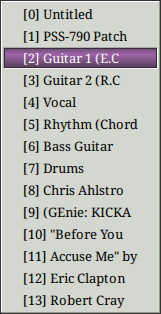
\includegraphics[scale=0.75]{pattern/background-sequence-menu.png}
   \caption{Sample Background Sequence Values}
   \label{fig:pattern_editor_background_sequence_menu}
\end{figure}

   Once the desired pattern is selected from that list, it appears as
   gray notes, along with the notes that are part of the pattern.  (Also
   note the orange selected notes and events in the following figure.)

\begin{figure}[H]
   \centering 
   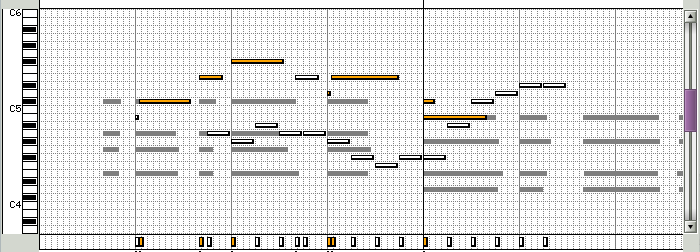
\includegraphics[scale=0.75]{pattern/background-sequence-notes.png}
   \caption{Background Sequence Notes}
   \label{fig:pattern_editor_background_sequence_notes}
\end{figure}

   The gray notes shown represent a rhythm pattern.

\subsection{Pattern Editor / Piano Roll}
\label{subsec:seq24_pattern_editor_piano_roll}

   The piano roll is the heart of the pattern (loop, sequence) editor.
   While it is very similar to note editors in other sequencers, it is a bit
   different in feel.  A good mouse with 3 or more buttons is practically a
   necessity for editing.  We tend to like the Logitech Marble Mouse, an
   ambidextrous USB trackball.  It has four bottons, and we use the
   \texttt{contrib/scripts/marblemouse} script to set up the left small
   button as a middle button.  The script merely makes the following call:

   \begin{verbatim}
      xmodmap -e "pointer = 1 8 3 4 9 6 7 2 5 10 11"
   \end{verbatim}

\subsubsection{Pattern Editor / Piano Roll Items}
\label{subsubsec:seq24_pattern_editor_piano_roll_items}

\begin{figure}[H]
   \centering 
   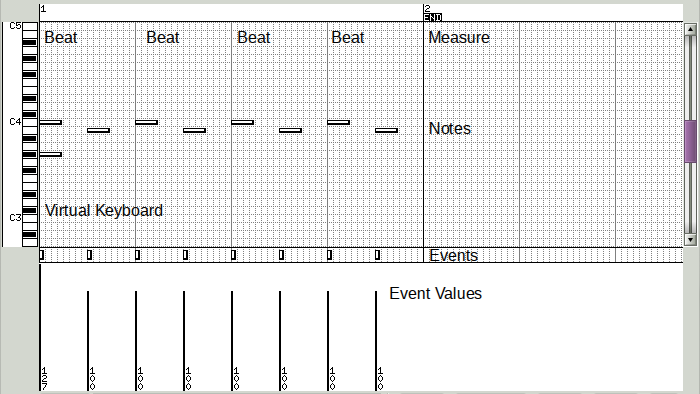
\includegraphics[scale=0.75]{pattern/pattern-edit-piano-roll-items.png}
   \caption{Pattern Editor, Piano Roll Items}
   \label{fig:pattern_editor_piano_roll_items}
\end{figure}

   \begin{enumber}
      \item \textbf{Beat}
      \item \textbf{Measure}
      \item \textbf{Virtual Keyboard}
      \item \textbf{Notes}
      \item \textbf{Events}
      \item \textbf{Event Values}
   \end{enumber}

   \setcounter{ItemCounter}{0}      % Reset the ItemCounter for this list.

   \itempar{Beat}{piano roll!beat}
   The light vertical lines represent the beats defined by the configuration
   for the pattern.

   \itempar{Measure}{piano roll!measure}
   The heavy vertical lines represent the measures defined by the
   configuration for the pattern.
   \index{pattern!end marker}
   Also note that the end of the pattern
   occurs at a measure, and is marked by a blocky \textbf{END} marker.

   \itempar{Virtual Keyboard}{piano roll!virtual keyboard}
   The virtual keyboard is a fairly powerful interface.  It shows,
   by shadowing, which note on the keyboard one will be drawing. It can be
   played with a mouse, to preview a short motif.
   It can show marks to indicate off-scale notes, to make them easy to
   avoid.

   \itempar{Notes}{piano roll!notes}
   Musical notes are indicated by short bars.  The bars provide a visual
   representation of the pitch of the note and the length of the notes.

   \itempar{Events}{piano roll!events}
   \index{events strip}
   The small (just a few pixels high) events strip shows discrete events,
   such as Note On and Note Off and their velocities, or various Controller
   items and their values.  We recommend not trying to edit or select events
   in that pane.

   \itempar{Event Values}{piano roll!event values}
   The events values for the currently selected category of events are shown
   in this window as vertical lines of a height proportional to the value.
   These values can be easily modified.

\subsubsection{Pattern Editor / Event Editing}
\label{subsubsec:seq24_pattern_editor_event_editing}

   Note editing is a bit different with \textsl{Seq24}, since it
   requires two mouse buttons in many cases.  There are some new
   laptop touchpads from FocalTech that have only one mouse button, and
   use positioning to determine if the click is a left- or right-click.
   The Linux drivers for this touchpad aren't sophisticated enough (as far
   as we know) to handle converting a two-fingered press properly.
   We've found that a good solution is to use a four-button USB trackball
   configued with an easy middle-button setup.
   It's easier than a touchpad, anyway.
   See the comments at the beginning of this section, too.

   Note that, if only a middle-button is needed, ctrl-left-button will
   simulate that button.

\paragraph{Editing Note Events}
\label{paragraph:seq24_pattern_editor_note_events}

   The Roll pane provides for a quite sophisticated set of note-editing
   actions.  Please study the following paragraphs carefully, ideally while
   trying them out in \textsl{Seq24}.

   \index{pattern editor!right click hold}
   \index{draw mode}
	In the note (grid/roll) panel, \textbf{holding}
	down the \textbf{right} mouse button will change the cursor
	to a pencil and put the editor into "draw" mode.
   
   \index{pattern editor!left click right hold}
   Then, while still \textbf{holding} the \textbf{right} mouse button, click
   the \textbf{left} mouse button to \textbf{insert} new notes.  Many people
   find this combination strange at first, but once one gets used to it, it
   becomes a very fast method of note manipulation.

   \index{pattern editor!right left hold drag}
   To increase the duration of the note(s), keep dragging the mouse (with
   both buttons held) rightward.
   \index{auto-notes}
   Note that, if one keeps dragging the mouse past the duration of a
   \index{beat unit}
   beat unit (e.g. a quarter note), then \textsl{multiple} notes are drawn,
   each one being the duration of a beat unit.  This \textsl{auto-note}
   facility can be convenient.
   
   However, if one wants a \textsl{single long note}, first draw the
   short note, and then use one of the operations described in the next
   paragraph to change the length of the note.  These operations also caused
   the note to be selected.

   \index{pattern editor!ctrl left click}
   \index{pattern editor!middle click}
   Pressing the \textbf{middle} mouse button \textbf{\textsl{or}}
   pressing the \textbf{ctrl left} mouse button tandem will let one change 
	the length of the note. 
   If more than one note is selected, then the length of all selected notes
   is changed.
   
   \textbf{Warning}:  If one reduces the length of a note by more than its
   current length, the note will end up "infinitely" long.

   \index{pattern editor!left click drag}
	The \textbf{left} mouse button lets you select multiple events 
   which can then be clicked and moved,
   \index{pattern editor!cut}
   \index{keys!ctrl-x} cut (\texttt{Ctrl-X}), 
   \index{pattern editor!copy}
   \index{keys!ctrl-c} copy (\texttt{Ctrl-C}),
   \index{pattern editor!paste}
   \index{keys!ctrl-v} or pasted (\texttt{Ctrl-V}).
   When the notes are selected,
   \index{pattern editor!delete}
   \index{keys!del} you can delete them with the \texttt{Delete} key.

   \index{ctrl left click drag}
   Pressing the \texttt{Ctrl} while left-click+dragging lets one
   make additional selections of multiple events and notes.

   For the appearance of selected events (orange), see
   \figureref{fig:pattern_editor_selected_events}.

\begin{figure}[H]
   \centering 
   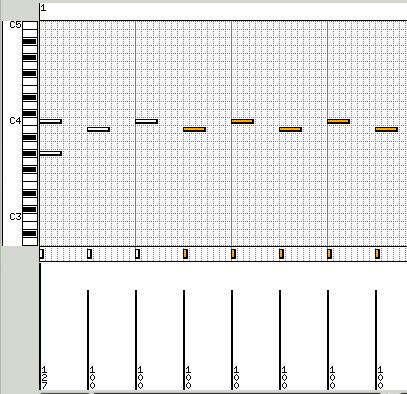
\includegraphics[scale=0.75]{pattern/pattern-edit-selected-events.png}
   \caption{Piano Roll, Selected Notes and Events}
   \label{fig:pattern_editor_selected_events}
\end{figure}

   \index{left click}
   Pressing the left button on a note or a event deselects all other notes
   or events, and selects the item clicked on.

   \index{ctrl left click}
   Pressing the \texttt{Ctrl} key and the left button on a note or a event
   \textsl{adds} that event to the selection.

   \index{left click drag}
   Note that pressing the left mouse button and dragging also lets one
   select multiple events and notes.
   \index{ctrl left click drag}
   Pressing the \texttt{Ctrl} while left-click+dragging lets one
   make additional selections of multiple events and notes.

   The \textbf{Tools} button described in
   \sectionref{subsec:seq24_pattern_editor_second} can also be used to
   modify selections.

   \index{keys!ctrl-a}
   \texttt{Ctrl-A} will select all of the events in the pattern editor.

   \index{pattern editor!ctrl left click}
   \index{pattern editor!middle click}
   Pressing the \textbf{middle} mouse button \textbf{\textsl{or}}
   pressing the \textbf{ctrl left} mouse button tandem will let one change 
	the length of the note. 
   If more than one note is selected, then the length of all selected notes
   is changed.

   \index{pattern editor!event stretch}
   \index{pattern editor!shift middle click drag}
   Once a selection of notes is made, one can use the
   Shift-middle-click+drag sequence over the selected notes to
   draw a box beyond the extent of the notes.  When the mouse is released,
   each of the events is moved and lengthed to be proporationally longer to
   fit exactly within the box one drew.
   This feature is called \textsl{event stretch}.

   \index{pattern editor!event compression}
   If the box that was drawn was shorter than the original extent of the
   notes, then the notes move and shrink proportionally to occupy the
   smaller box.
   This feature is called \textsl{event compression}.
   
   \textbf{Warning}:  If one reduces the length of a note by more than its
   current length, the note will end up "infinitely" long.

   \index{pattern editor!left click drag}
	The \textbf{left} mouse button lets you select multiple events 
   which can then be clicked and moved,
   \index{pattern editor!cut}
   \index{keys!ctrl-x}
   cut (\texttt{Ctrl-X}), 
   \index{pattern editor!copy}
   \index{keys!ctrl-c}
   copy (\texttt{Ctrl-C}),
   \index{pattern editor!paste}
   \index{keys!ctrl-v}
   or pasted (\texttt{Ctrl-V}).
   When the notes are selected,
   \index{pattern editor!delete}
   \index{keys!del}
   you can delete them with the \texttt{Delete} key.

\paragraph{Editing Other Events}
\label{paragraph:seq24_pattern_editor_other_events}

%  Left-click or right-click on events in the event strip (directly under
%  the piano roll grid) will allow you to add/select/move 
%  MIDI events (including note on/off messages) somewhat like the 
%  piano grid.

   \index{event strip}
   Note On and Note Off events appear as small squares in the event strip,
   along with a black vertical bar with a height proportional to the
   velocity of the note event, plus a numeric representation of that value.
   Note events do not need to be inserted in the event strip.
   (\textsl{Note events can be inserted there, but they end up as short
   events of the lowest possible note, 0 or C1, and they don't have a Note
   Off event.  So don't do that!})

   Other events can be inserted via the event strip.  To do that, first
   select the kind of event to insert using the \textbf{Event} button in the
   bottom panel.  The place the mouse cursor in the event strip.
   Right-click to make the drawing pencil appear at the exact spot where the
   event must go.  While holding the right button, click the left button.
   A small square for the event should appear.

   Should one want more of the same event, continue to hold both buttons and
   drag the mouse.  One event should appear at each beat position (e.g. at
   each 16th note position) that is crossed.

   To move the event(s) to a different spot, select it or them via the left
   button.  Then drag it or them to where one wants them.
   \index{todo!high precision events}
   \textsl{Note: it
   is currently not possible to move them to positions smaller than the
   beat size.  Is there a way to do it?}

   Once the event positions are set, the next step is to modify the
   data values of the events.

   \index{event data}
	The event value (data) editor (directly under the event strip) is used 
	to change note velocities, channel pressure, control codes,
	patch select, etc.
   \index{event data editor!draw}
   \index{event data editor!left click}
   \index{event data editor!right click}
   \index{event data editor!middle click}
   Just left-click+drag the mouse across the window to draw a line.  The
   values will match that line.  
   middle-click+drag and right-click+drag also
   draw the value line.

   \textbf{Bug:}
   \index{bugs!event editing can fail}
   Sometimes the editing of event values in the event data section will not work.
   The workaround is to do a \texttt{Ctrl-A}, and the click in the roll
   to deselect the selection; that makes the event value editing work again.
   
   \index{event data editor!mouse wheel}
   Any events that are selected in the piano roll or event strip can have
   their values modified with the mouse wheel.

\subsection{Pattern Editor / Bottom Panel}
\label{subsec:seq24_pattern_editor_bottom}

   The bottom panel of the Pattern Editor provides for selecting events for
   viewing and edition, and the MIDI playback, pass-through, and recording
   options of \textsl{Seq24}.

\begin{figure}[H]
   \centering 
   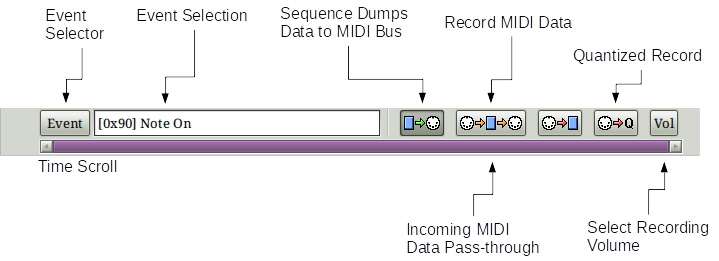
\includegraphics[scale=0.75]{pattern/pattern-edit-bottom-panel-items.png}
   \caption{Pattern Editor, Bottom Panel Items}
   \label{fig:pattern_editor_bottom_panel_items}
\end{figure}

   \begin{enumber}
      \item \textbf{Event Selector}
      \item \textbf{Event Selection}
      \item \textbf{Time Scroll}
      \item \textbf{Data To MIDI Buss}
      \item \textbf{MIDI Data Pass-Through}
      \item \textbf{Record MIDI Data}
      \item \textbf{Quantized Record}
      \item \textbf{Select Recording Volume}
   \end{enumber}

   \setcounter{ItemCounter}{0}      % Reset the ItemCounter for this list.

   \itempar{Event Selector}{pattern editor!event selector}
   This button brings up the following context menu, so that the user can
   select the category of events to view and edit.

\begin{figure}[H]
   \centering 
   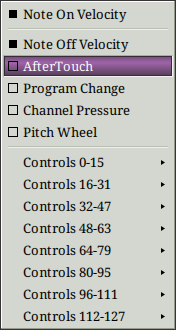
\includegraphics[scale=0.75]{pattern/event-context-menu.png}
   \caption{Pattern Editor, Event Button Context Menu}
   \label{fig:pattern_editor_bottom_event_context_menu}
\end{figure}

   The sub-menus of this context menu show 128 controller messages,
   so we won't try to show all of them here.

   These sub-menus can be modified, as far as we know, by editing
   the file \texttt{\$HOME/.seq24usr}, to make it match your instrument.
   See \sectionref{sec:seq24_usr_file}.

   \itempar{Event Selection}{pattern editor!event selection}
   Shows the selection event, with its number shown in hexadecimal notation,
   and the name of the event shown.

   \itempar{Time Scroll}{pattern editor!time scroll}
   Allows one to pan through the whole pattern, if it is too long to fit in
   the window.

   \itempar{Data To MIDI Buss}{pattern editor!data to midi buss}
   Activating this button will cause the pattern to be output to the MIDI
   output buss, which will normally be connected to a software or hardware
   synthesizer, to be heard.

   \itempar{MIDI Data Pass-Through}{pattern editor!midi data pass-through}
   Activating this button will route incoming MIDI data through
   \textsl{Seq24}, which will then write it to the MIDI output buss.

   \itempar{Record MIDI Data}{pattern editor!record midi data}
   Activating this button will route incoming MIDI data into
   \textsl{Seq24}, which will then save the data to its buffer, and also
   display the new information (notes) in the piano roll view.

   \itempar{Quantized Record}{pattern editor!quantized record}
   Activating this button will also cause MIDI data to be recorded, but it
   will be quantized on the fly before saving it.

   \itempar{Vol}{pattern editor!vol}
   This button allows controlling the volume of the recording.

\begin{figure}[H]
   \centering 
   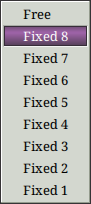
\includegraphics[scale=0.75]{pattern/vol-context-menu.png}
   \caption{Pattern Recording Volume Menu}
   \label{fig:pattern_edit_recording_volume_menu}
\end{figure}

   The values provided are:
   Free, Fixed 8, Fixed 7, Fixed 6, Fixed 5, Fixed 4, Fixed 3,
   Fixed 2, and Fixed 1.
   TODO: \index{todo!explain recording volume}
   We need to figure what these mean!

%-------------------------------------------------------------------------------
% vim: ts=3 sw=3 et ft=tex
%-------------------------------------------------------------------------------
